Tato kapitola rozebírá, k~čemu slouží zaznamenávání odpracovaného času. Poté popisuje možnosti, které umožňují měření času spouštět a také se věnuje příkladům řešení, která již pro zaznamenávání odpracovaného času existují. V dalších sekcích se poté obecně zaměřuje na vývoj aplikací pro mobilní platformu iOS včetně možností multiplatformního a cross-platformního vývoje. Na závěr poté zkoumá, jaké existují možnosti pro integraci spouštěčů měření odpracovaného času a exportu dat do dalších aplikací.

%---------------------------------------------------------------
\section{Zaznamenávání odpracovaného času}
%---------------------------------------------------------------

Zaznamenávání odpracovaného času může být potřeba z~několika různých důvodů, buď z~pohledu jednotlivce, nebo z~pohledu spolupráce v~nějakém týmu. Mezi tyto důvody může patřit například:
\begin{itemize}
\item\textbf{Sledování pracovních hodin:} Pomáhá zaměstnancům a podnikům sledovat, kolik času strávili na různých úkolech, projektů a aktivitách během pracovní doby. To může být užitečné pro sledování produktivity, hodnocení efektivity práce a plánování rozpočtu času.
\item\textbf{Fakturace a účtování:} Pro profesionály a firmy, které účtují za své služby na základě odpracovaného času, umožňuje zaznamenávání snadné sledování času stráveného na jednotlivých projektech a klientech pro účely fakturace.
\item\textbf{Analýza produktivity:} Poskytuje data a statistiky o~tom, jaký čas je věnován různým úkolům a projektům. To umožňuje identifikovat trendy v~pracovních návycích, optimalizovat časové plánování a zlepšit efektivitu práce.
\item\textbf{Správa projektů:} Pomáhá organizovat časové údaje spojené s~různými projekty a úkoly, což usnadňuje plánování, delegování a monitorování pokroku.
\item\textbf{Transparentnost a komunikace:} Pro týmy umožňuje transparentně sdílet informace o~čase stráveném na různých aktivitách, což podporuje spolupráci a komunikaci v rámci týmu.
\end{itemize}

Celkově zaznamenávání slouží k~lepšímu řízení času, sledování produktivity a optimalizaci využití pracovního času pro jednotlivce i~organizace.

\begin{figure}[h]
	\centering
	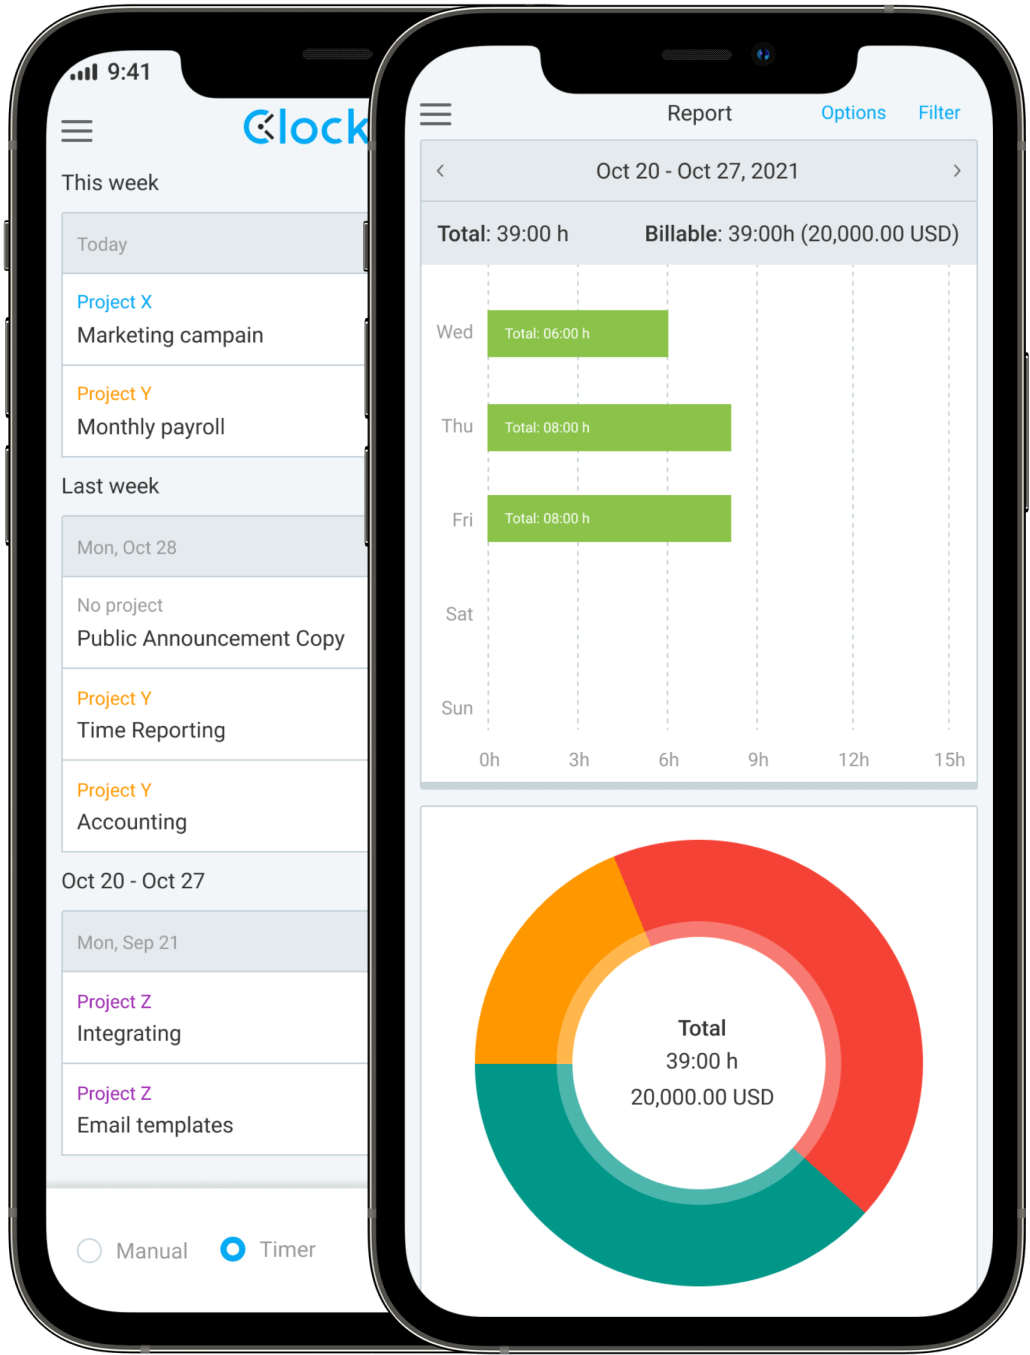
\includegraphics[width=10cm]{clockify-ios.png}
	\caption{Clockify – iOS aplikace pro měření času \cite{clockify-ios}}
	\label{fig:clockify-ios}
\end{figure}

%---------------------------------------------------------------
\section{Spouštěče měření času}
%---------------------------------------------------------------

Jedním z~cílů této práce je prozkoumat různá řešení pro spouštěče měření času. Nejjednodušším spouštěčem je samozřejmě ruční zapnutí nějaké formy časovače v~samotné aplikaci, která pro měření času slouží. To ale umí kdejaké již existující řešení a přidanou hodnotou této práce by měly být nějaké možnosti, jak spouštění uživateli ulehčit. Tyto možnosti se dají rozdělit do dvou kategorií – fyzické a softwarové.

%---------------------------------------------------------------
\subsection{Fyzické}
%---------------------------------------------------------------

Za fyzické spouštěče měření času lze považovat jakoukoli formu fyzického ovladače, kterou může uživatel nějak ovládat a tím spouštět časovač měření času.

Častým typem fyzického spouštěče je nějaká forma takzvaného platónského tělesa (krychle, osmistěn, dvanáctistěn, atd.), které může uživatel otáčet. Podle toho, na kterou stranu ho položí, tak se spustí časovač s danými parametry. Různé strany tělesa mohou sloužit například pro identifikování toho, na kterém projektu uživatel zrovna pracuje.

Mezi fyzické spouštěče patří například tyto produkty:
\begin{itemize}
\item\textbf{TIMEFLIP:} Dvanáctistěnné těleso, na které si uživatel může nalepovat cokoli, co bude identifikovat odpracovaný čas. Těleso se propojí s~mobilní aplikací, která poté spravuje naměřený čas. \cite{timeflip}
\item\textbf{TIMEULAR:} Stejný princip jako TIMEFLIP, akorát používá osmistěnné těleso. Jednotlivé strany jdou také přizpůsobovat nálepkami. \cite{timeular}
\item\textbf{timeBuzzer:} Fyzické tlačítko, které lze umístit na stůl a zapojit do počítače. Stisknutí tlačítka otevře okno měřící aplikace, otočením tlačítka lze vybrat projekt a opětovným stisknutím se začne daný projekt měřit. \cite{timebuzzer}
\end{itemize}

\begin{figure}[h]
	\centering
	\begin{subfigure}[b]{5.2cm}
		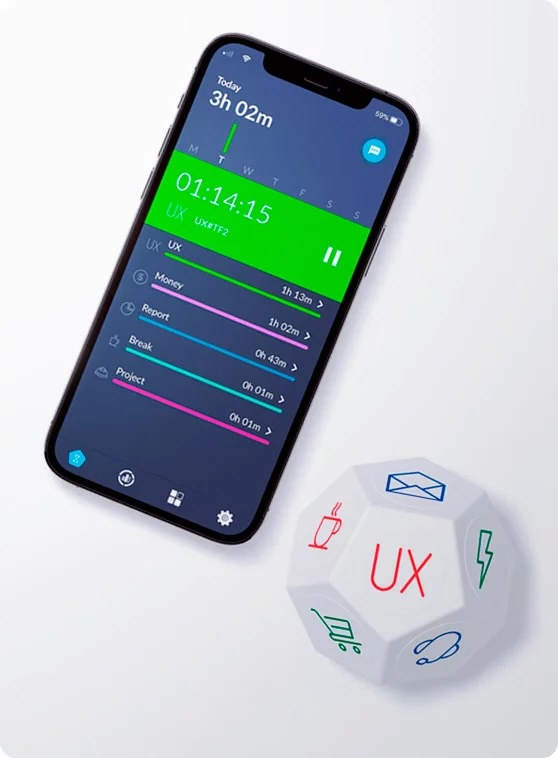
\includegraphics[width=5.2cm]{timeflip.jpeg}
		\caption{TIMEFLIP – Kostka a aplikace \cite{timeflip}}
		\label{pic:timeflip}
	\end{subfigure}
	\hspace{2cm}
	\begin{subfigure}[b]{7cm}
		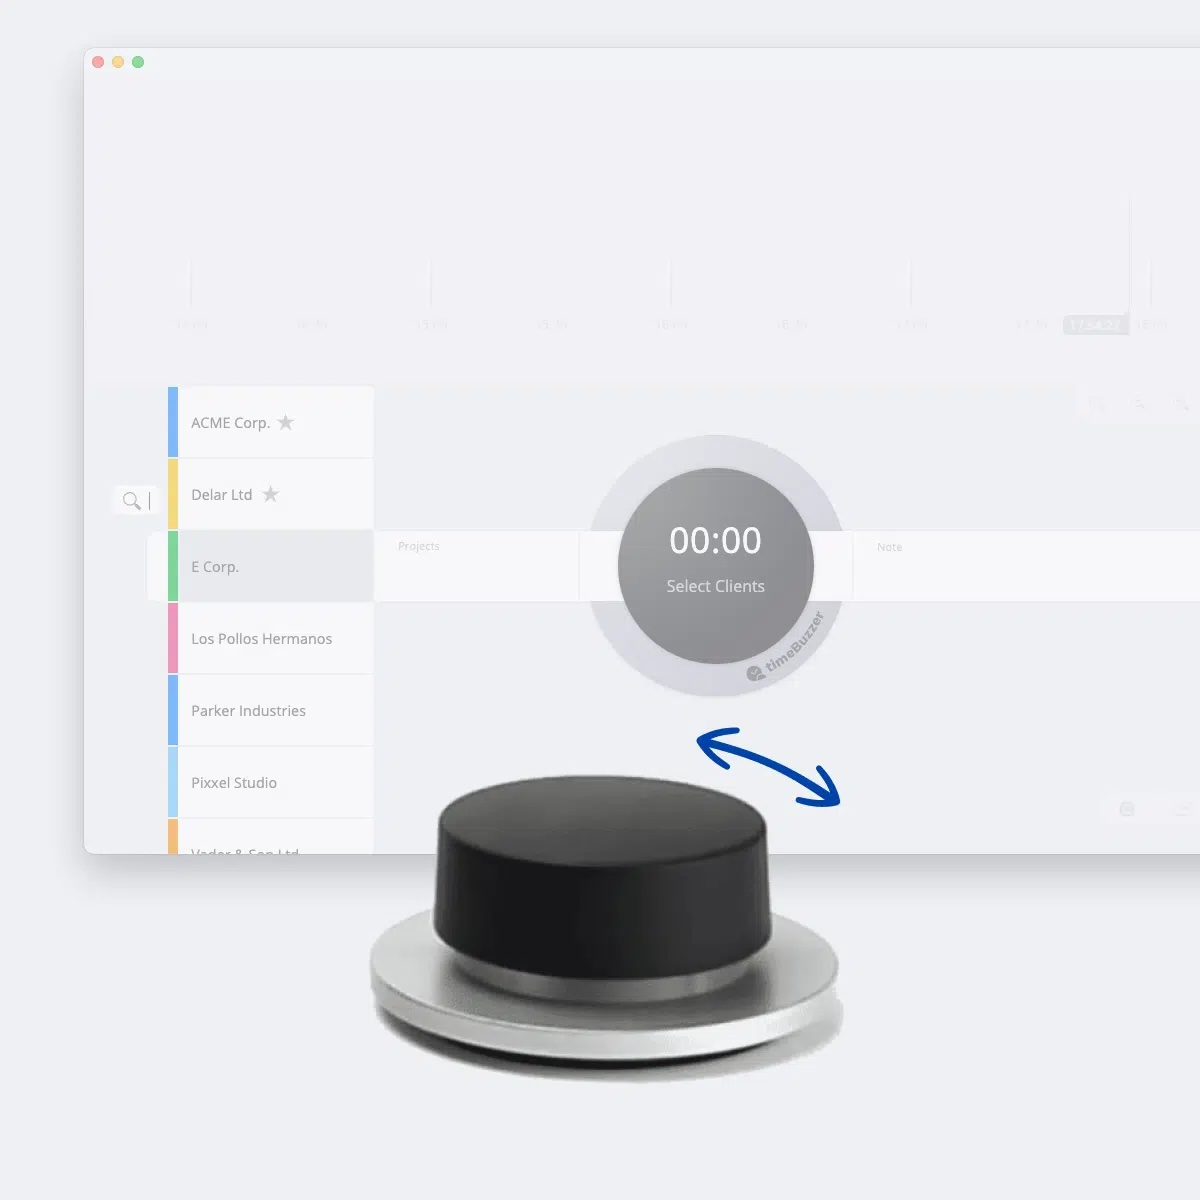
\includegraphics[width=7cm]{timebuzzer.jpeg}
		\caption{timeBuzzer – tlačítko a aplikace \cite{timebuzzer}}
		\label{pic:timebuzzer}
	\end{subfigure}
\end{figure}

Všechny ze zmíněných produktů poskytují veřejné API pro aplikace, se kterými komunikují \cite{timeflip-api} \cite{timeular-api} \cite{timebuzzer-api}. Pokud by tedy bylo potřeba produkty propojit s~vlastní aplikací, která by mohla naměřený čas spravovat, bylo by potřeba, aby aplikace komunikovala s~těmito nástroji. Pořád by byl potřeba prostředník, kterým by byla aplikace daného produktu. Výjimkou je v~těchto produktech pouze TIMEFLIP, který poskytuje veřejný protokol pro BLE komunikaci \cite{timeflip-ble-api}. Tento produkt by tedy mohl komunikovat s~novou aplikací napřímo.

Pokud by nová aplikace měla umožňovat budoucí propojení s~jakýmkoli dalším hardwarovým produktem, tak by také měla poskytovat veřejné API, které by takovou komunikaci umožňovalo. Vývoj takových produktů by mohl být předmětem návrhu pro budoucí vylepšení aplikace.

%---------------------------------------------------------------
\subsection{Softwarové}
%---------------------------------------------------------------

Za softwarové spouštěče měření času lze považovat určité formy integrace a automatizace v~rámci zařízení, na kterém aplikace běží. V~případě aplikace na platformě iOS to mohou být následující možnosti:
\begin{itemize}
\item\textbf{Automatizace podle polohy:} Aplikace by mohla reagovat na polohu uživatele a spouštět nebo vypínat časovač na základně informace, kde se uživatel nachází. Uživatel by si mohl například nastavit určitá místa, kde by chtěl, aby se automaticky spustil časovač. Mohl by se zapnout přímo s~konkrétními přednastavenými parametry (projekt, klient, \dots), nebo by se jen mohlo ukázat upozornění, aby si uživatel časovač zapl sám, s~parametry, které zadá. Podobně by aplikace mohla reagovat i na opuštění nějakého místa – například pokud uživatel opustí místo, které má označeno jako práci, tak by dostal upozornění, zda si nechce vypnout časovač.
\item\textbf{Automatizace podle času:} Jednoduchá forma automatizace by mohla fungovat na základě času. V~přednastavených časech by se mohl zapnout nebo vypnout časovač s~danými parametry, nebo by aplikace mohla uživatele jen upozornit.
\item\textbf{Automatizace podle kalendáře:} Užitečná by také mohla být integrace s~kalendářem uživatele. Podle naplánovaných událostí by se časovač mohl automaticky zapínat, přepínat, nebo vypínat, s~parametry z~kalendáře. Nebo opět pouze uživatele upozornit, zda si kvůli nějaké události nechce měření času aktualizovat.
\end{itemize}
